\section{Modelling the Earth}

\subsection{Global Models}

 Earth Simpulation Models (ESM) are models which predict past or future interactions of the planetary system. They represnt our foremost understanding of the complex interplay between land-surface (geosphere), ocean (hydrosphere), ice (cryosphere) and the air (atmosphere). These act as a surrogate to manual experimentation, which is just not possible on the global scle, and enable us to access changes, situations and predict the future. 

Earth simulation models often have to address many problems relating to computational efficiency.  
% 
% \subsubsection{Common Problems with Earth prediction}
% There are several problems that an earth simulation model can face, most of which can be attributed to computational efficiency. An example of this is seen with the 
% 
% MET - DAY TO SIMULATE
% 
% Other problems with meteorlogy that are encountered rest on resolution. Too fine a scale and the model can take forever to run. simplfy, lose local effect and islands. 
% 
% Finally the tuning of models can result in overfitting due to a limited understanding or dataset. Here a model may be tweked to .. 
% 
% Numerical stiff chemical complexity. 
% 
% 


\subsection{The Atmosphere}

\subsubsection{Types of model}
3d transoport emission/deposition chemical and physical processes 




\subsubsection{Chemical Mechanisms}
The atmosphere consists of thousands of species, with tens of thousands of reactions between them. Since manual experimentation is not possible on both the macro (every location on earth) or micro (every atom) scale for the Earth System any prediction of these requires the use of a numerical model. 


These models represent real wodlc reactions 


In modelling these we can describe their rate of production and loss with respect to the species they react with. 



\subsection{The model development cycle}
Scientific understanding is the product of many cycles of trial and error, \autoref{fig:devcycle}. In atmospheric chemistry we start with a hypothesis or a question, e.g. will changing X have a negative response on Y. We then construct a theoretical model to represent the chemsistry within. This chemistry is updated to reflect the rates and reactions that have been recorded in laboratory/chamber experiments. This cycle is then repeated until the model and real-world observations produce a comparable result. 

\begin{figure}[H]
    \centering
    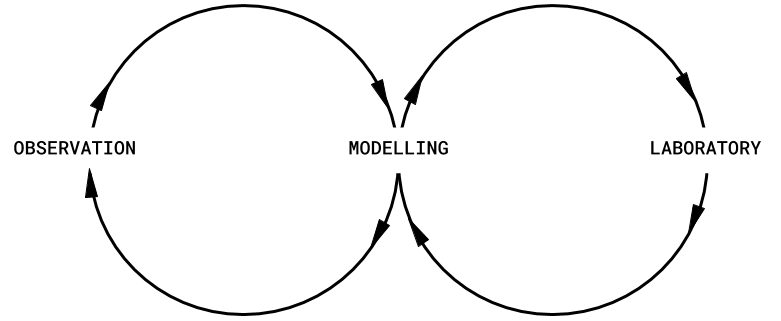
\includegraphics[width=0.6\textwidth]{devcycle.png}
    \caption{\textbf{The scientific development cycle.}This shows the iterative nature between modelling, observation and laboratory experimentation}
    \label{fig:devcycle}
\end{figure}






ESM 

 A series of box models.
 
 
 \subsection{The Dynamically Simple Model of Atmospheric Chemical Complexity}
 
 





